\chapter{Applicazione di SFA: La Tramvia di Firenze}
In questo capitolo verr\`a analizzata una particolare applicazione di un KF al problema del posizionamento ferrotramviario.\\*
Nell'ambito di un progetto di ricerca finanziato dall'Unione Europea, si \`e voluto studiare l'usabilit\`a di KF come sistema di posizionamento ferrotramviario alternativo a quello descritto nel Capitolo 1, il quale fa un largo uso di apparati installati a terra, fatto che si vorrebbe minimizzare.\\*
La linea ferrotramviaria scelta come ambiente di prova \`e la linea \texttt{T1} della Tramvia di Firenze, che collega la stazione di \emph{Villa Costanza}, sita nel comune di Scandicci all'altezza dell'omonimo parcheggio di interscambio dell'autostrada \texttt{A1}, all'ospedale di \emph{Careggi}, sito quest'ultimo nel comune di Firenze.
\begin{figure}[h]
	\centering
	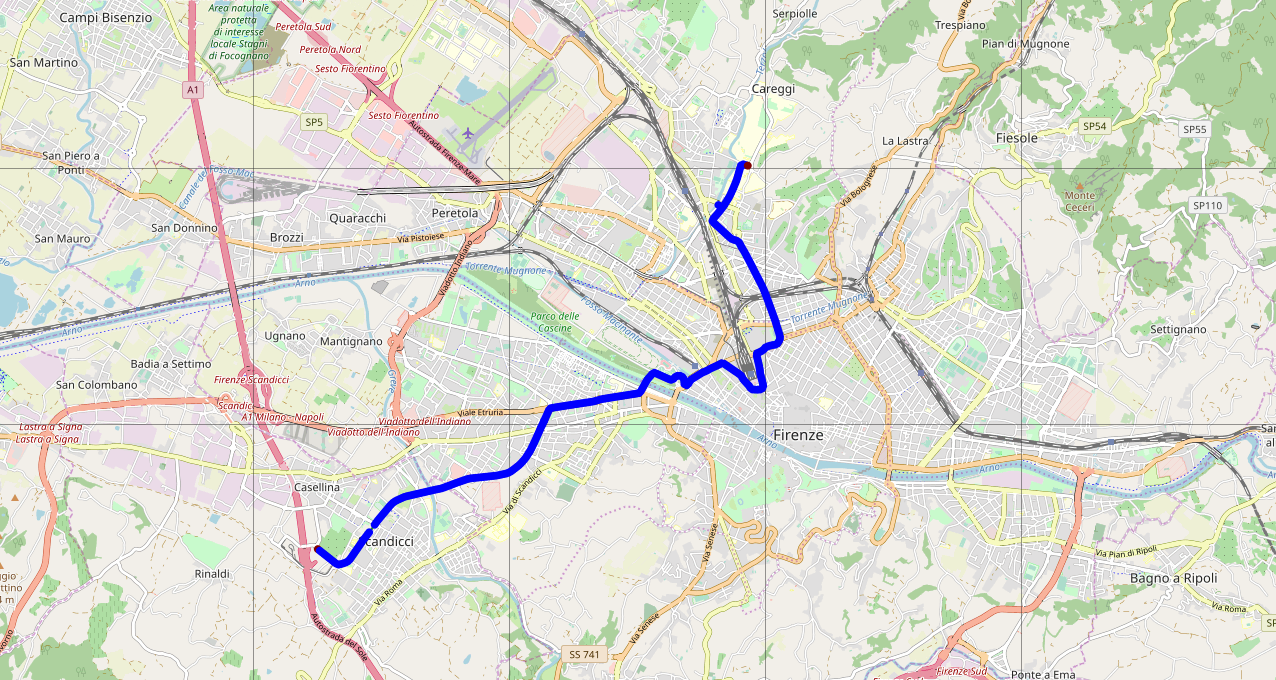
\includegraphics[width=\linewidth]{img/t1}
	\caption{Tramvia di Firenze - Linea \texttt{T1}}
	\label{fig:t1}
\end{figure}
\section{Architettura di Sistema}
Il sistema progettato ha lo scopo di eseguire SFA su una piattaforma hardware installata bordo treno, la quale riceve i dati \emph{raw} dai sensori e li elabora al fine di stimare la progressiva chilometrica del treno in ciascun istante di tempo.\\*
Tale posizione sar\`a inviata, attraverso un modem \texttt{LTE}:
\begin{itemize}
	\item All'OBCU, per essere utilizzata attivamente all'interno del sistema di \emph{interlocking}
	\item Ad un arbitario host che esegue un software grafico di tracciamento del treno: il \texttt{RailTrackTool} (RTT)
\end{itemize}
\`E possibile descrivere l'architettura di sistema a due differenti livelli: architettura a livello \emph{hardware} e architettura a livello \emph{software}.\\*
\subsection{Architettura Hardware}
Sul treno \`e stata installata una scheda \texttt{Nvidia TX-Jetson} quale piattaforma di elaborazione dei dati. I sensori atti a campionare le misurazioni sono stati collegati alla scheda mediante appositi bus dati.\\*
Il \emph{sensor set} utilizzato in quest'applicazione \`e composto dai seguenti sensori:
\begin{itemize}
	\item \emph{Inertial Measurement Unit} (IMU):\\*
	Unit\`a incaricata di misurare i vettori \texttt{accelerazione} ($\mathbf{a}$) e \texttt{velocit\`a angolare} ($\mathbf{v_{ang}}$) attraverso l'uso combinato di un accelerometro e un giroscopio. Le misure di IMU sono prese rispetto a un sistema inerziale solidale con il binario e sono espresse in unit\`a stabilite dallo standard internazionale (SI):
	$$
	\mathbf{a}\;\left[\frac{m}{s^2}\right]\;\;\;\;\mathbf{v_{ang}}\;\left[ \frac{rad}{s} \right]
	$$Si tratta del sensore principale su cui si basa l'esecuzione di SFA.\newpage
	\item Odometro:\\*
	Per realizzare l'odometro \`e stato installato un rilevatore radar su una ruota del treno. Il radar misura il tempo impiegato dalla ruota a compiere un giro completo, e determina la velocit\`a angolare della ruota $\varphi'(t) = \frac{2\pi}{tempo} \left[ \frac{rad}{s}\right]$.\\*
	Noto il raggio $r\;[m]$ della ruota, \`e possibile determinare la velocit\`a lineare alla circonferenza della ruota  $x'(t)$ attraverso la relazione cinematica $x'(t) = r\varphi'(t) \left[ \frac{m\;rad}{s}\right] = r\varphi'(t) \left[ \frac{m}{s} \right]$.\\*
	Approssimando il treno come un \emph{corpo rigido}, questa sar\`a la velocit\`a lineare con cui il treno si sta muovendo.
	\item Global Positioning System (GPS):\\*
	Modulo che riceve i dati di posizione attraverso il sistema satellitare GPS.\\*
	Le misure di GPS sono riportate in formato standard come tripla di coordinate \texttt{(latitudine, longitudine, altitudine)}, rispettivamente espresse in gradi \texttt{N-S}, in gradi \texttt{E-O} e in \texttt{metri}.\\*
	In generale queste misure sono le meno affidabili in quanto la \emph{varianza} della variabile aleatoria che modella tale sorgente \`e la pi\`u significativa.
\end{itemize}
 Ad una data frequenza, i sensori inviano dati verso la scheda; quest'ultima, dopo aver eseguito un'iterazione di SFA, invia a OBCU (e/o a RTT) la stima della posizione del treno attraverso apposita modulazione di segnale elettromagnetico, in accordo con il protcollo \texttt{LTE}. Lo schema riportato in figura \ref{fig:tdiagram} mostra un diagramma dell'architettura hardware appena descritta.
\begin{figure}[h]
	\centering
	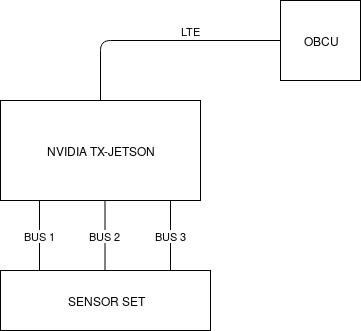
\includegraphics[width=0.7\linewidth]{img/TrainDiagram}
	\caption{Architettura hardware bordo treno}
	\label{fig:tdiagram}
\end{figure}
\subsection{Architettura Software}
Sulla scheda \`e installato il sistema operativo \texttt{Ubuntu 16.04 LTS}, basato su kernel \texttt{Linux}.\\*
Un set di tre moduli software, denominati \texttt{interface-modules}, sono in esecuzione sulla scheda.\\*
Sia MOD\_$i$ l'$i-$esimo modulo del set e SERIAL\_$i$ l'$i-$esima interfaccia seriale della scheda, per $i = 1,2,3$.\\*
Il funzionamento di \texttt{interface-modules} \`e il seguente
\begin{itemize}
	\item IMU invia la coppia \texttt{(accelerazione,velocit\`a angolare)} a SERIAL\_1, MOD\_1 legge i valori da SERIAL\_1 e li invia a un secondo modulo software, denominato \texttt{listener}, attraverso l'interfaccia di rete \texttt{loopback}, in quanto \texttt{listener} esegue anch'esso sulla scheda;
	\item Odometro invia il valore di \texttt{velocit\`a lineare} a SERIAL\_2, MOD\_2 legge i valori da SERIAL\_2 e li invia a \texttt{listener}
	\item GPS invia il vallore di \texttt{(latitudine, longitudine, altitudine)} a SERIAL\_3, MOD\_3 legge i valori da SERIAL\_3 e li invia a \texttt{listener}
\end{itemize}
La comunicazione fra \texttt{interface-modules} e \texttt{listener} avviene attraverso un protocollo applicazione stabilito arbitrariamente, sia esso \texttt{INPUT\_PROTOCOL}, mentre a livello di trasporto si utilizza \texttt{UDP}.\\*
I valori ricevuti da \texttt{listener} vengono salvati in apposite \emph{strutture dati} rappresentanti misure della stessa sorgente:
\begin{itemize}
\item I vettori accelerazione e velocit\`a angolare rilevati da IMU vengono convertiti nella struttura dati \texttt{IMU\_POD};
\item La velocit\`a rilevata dal Radar/Odometro viene convertita nella struttura dati \texttt{ODO\_POD};
\item La posizione rilevata dal GPS viene infine convertita nella struttura dati \texttt{GPS\_POD}.
\end{itemize}
Il software che esegue effettivamente SFA \`e compilato come una libreria, \texttt{FusionLib}, utilizzata da \texttt{listener}. \texttt{FusionLib} dispone di interfacce software in entrata e in uscita, ossia \texttt{listener} \`e in grado di inviare le misurazioni a SFA, quali variabili di tipo \texttt{IMU\_POD, ODO\_POD, GPS\_POD} ed altres\'i di ricevere la stima della posizione del treno, essendo questo l'output dell'algoritmo, quale variabile di tipo \texttt{SFA\_OUTPUT\_POD}.\\*
Ogniqualvolta \texttt{listener} riceva un' uscita da SFA, esso si fa carico della comunicazione tra scheda e OBCU (oppure tra scheda e RTT). Questa comunicazione, fisicamente possibile attraverso l'utilizzo del modem \texttt{LTE}, avviene utilizzando un protocollo di rete arbitrario a livello applicazione, sia esso \texttt{OUTPUT\_PROTOCOL}, mentre al livello di trasporto la scelta \`e nuovamente ricaduta su \texttt{UDP} per ragioni di efficienza.\\*
Si osserva che \texttt{INPUT\_PROTOCOL} e \texttt{OUTPUT\_PROTOCOL} sono entrambi protocolli arbitrari a livello applicazione, ma necessariamente differenti. Questo aspetto verr\`a discusso nella prossima sezione. Uno schema dell'architettura software \`e quello mostrato in figura \ref{fig:tdiagramint}.\\*
\begin{figure}[h]
	\centering
	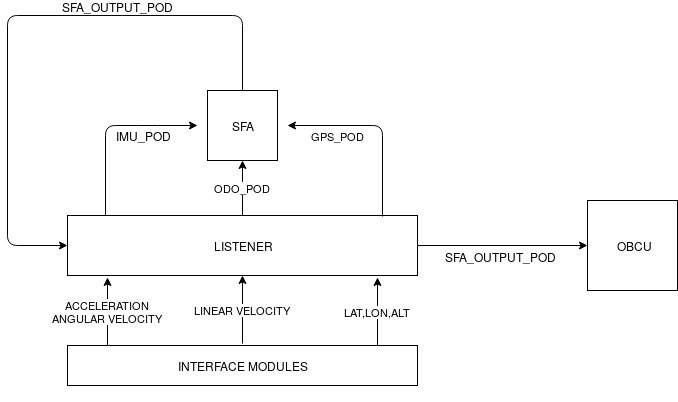
\includegraphics[width=\linewidth]{img/InternalTrainSchema}
	\caption{Architettura software bordo treno}
	\label{fig:tdiagramint}
\end{figure}
\section{Gestione della trasmissione dei dati}
Per trasmettere i dati da \texttt{interface-modules} a \texttt{listener} \`e stato implementato un protocollo di comunicazione denominato \texttt{INPUT\_PROTOCOL}.\\*
Tale protocollo fa affidamento a livello trasporto su \texttt{UDP} per massimizzare la velocit\`a di trasmissione senza dover necessariamente rinunciare all'integrit\`a dei messaggi trasmessi, in quanto la comunicazione avviene tra processi in esecuzione sulla stessa macchina, e la probabilit\`a che un messaggio venga perso o che questo venga ricevuto con errori, \`e assolutamente trascurabile.\\*
Il protocollo definisce il formato del \emph{payload} del pacchetto \texttt{UDP} che contiene le informazioni di IMU, Radar/Odometro, o GPS, ed \`e il seguente:



